\documentclass[tikz, border=10pt]{standalone}

\usepackage{tikz}
\usepackage{palatino}
%\usepackage[no-math]{fontspec}
% \setmonofont{Fira Code}


\newcommand{\headerbox}[7]{
    \begin{scope}[shift={(#1,#2)}]
        \def\boxWidth{#6}
        \def\headerHeight{1cm}
        \def\mainHeight{#7}

        % Draw the main box and name it with the fifth argument
        \draw (0,0) rectangle (\boxWidth,\mainHeight) coordinate (#5-main);
        \node[anchor=north west, align=left, text width=\boxWidth-1em, yshift=-1ex, xshift=0.5ex] (main) at (0,\mainHeight) {#3};

        % Draw the header box and name it with the fifth argument
        \draw (0,\mainHeight) rectangle (\boxWidth,\mainHeight+\headerHeight) coordinate (#5-header) 
        node[midway, align=left, text width=\boxWidth-1em] (header) {\textbf{#4}};
    \end{scope}
}

\begin{document}
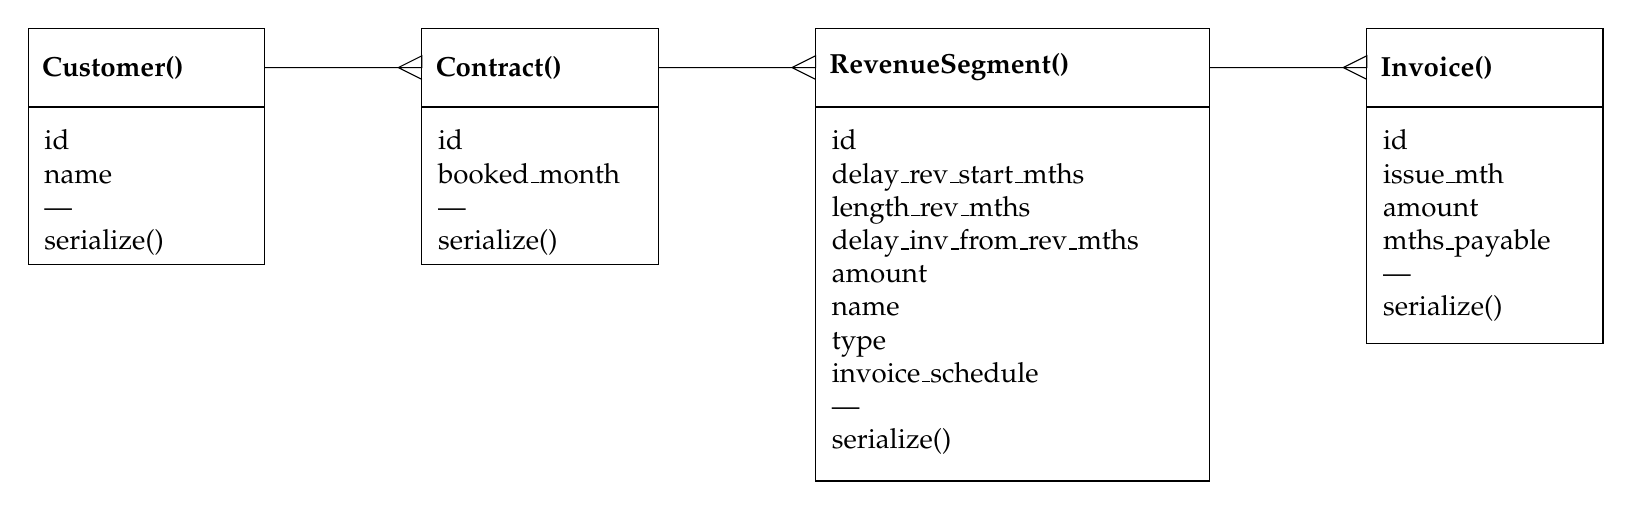
\begin{tikzpicture}

%  \draw[step=1cm, gray!30, ultra thin] (0,-5) grid (22,5);
  
    \headerbox{0}{0}{id\\name\\---\\serialize()}{Customer()}{box1}{3cm}{2cm}
    \headerbox{5}{0}{id\\booked\_month\\---\\serialize()}{Contract()}{box2}{3cm}{2cm}
    \headerbox{10}{-2.75}{id\\delay\_rev\_start\_mths\\length\_rev\_mths\\delay\_inv\_from\_rev\_mths\\amount\\name\\type\\invoice\_schedule\\---\\serialize()}{RevenueSegment()}{box3}{5cm}{4.75cm}
    \headerbox{17}{-1}{id\\issue\_mth\\amount\\mths\_payable\\---\\serialize()}{Invoice()}{box4}{3cm}{3cm}
    
    \draw (3,2.5) -- (5,2.5) -- ++(0cm,0.15cm) -- ++(-0.3cm,-0.15cm) -- ++(0.3cm,-0.15cm);
    
    \draw (8,2.5) -- (10,2.5) -- ++(0cm,0.15cm) -- ++(-0.3cm,-0.15cm) -- ++(0.3cm,-0.15cm);
    \draw (15,2.5) -- (17,2.5) -- ++(0cm,0.15cm) -- ++(-0.3cm,-0.15cm) -- ++(0.3cm,-0.15cm);
\end{tikzpicture}
\end{document}


%%% Local Variables:
%%% mode: latex
%%% TeX-master: t
%%% End: